\documentclass{report}

\input{preamble}
\input{macros}
\input{letterfonts}

\title{\Huge{MAM2000W}\\Linear Transformations}
\author{\huge{Alex Cristaudo}}
\date{}

\begin{document}

\maketitle
\newpage% or \cleardoublepage
% \pdfbookmark[<level>]{<title>}{<dest>}
\pdfbookmark[section]{\contentsname}{toc}
\tableofcontents
\pagebreak



\chapter{Linear Transformations}
\section{Linear Transformations}
\dfn{}{
    Let $T$ be a function from vector space  $V$ to vector space  $W$. We say that  $T$ is a linear transformation if it satisfies 2 conditions:
     \begin{itemize}
        \item $T(\mathbf{u}+\mathbf{v}) = T(\mathbf{u}) + T(\mathbf{v})$ for every $\mathbf{u}, \mathbf{v} \in V$
        \item $T( \lambda \mathbf{u}) = \lambda T(\mathbf{u})$ for every scalar $ \lambda $ and vector $\mathbf{u} \in V$
    \end{itemize}
}

\ex{}{
 Let $A = \begin{pmatrix} 1  & 2 & 3 \\ 1 & -3 & 2 \end{pmatrix} $. For every $ \mathbf{x} = \begin{pmatrix} x_1 \\ x_2 \\ x_3 \end{pmatrix} \in \mathbb{R}^3$, let 
 \begin{center}
     $T(\mathbf{x}) = A \mathbf{x} = \begin{pmatrix} x_1+2x_2+3x+3 \\ x_1-3x_2+2x_3 \end{pmatrix} $
 \end{center}
 This $T$ defines a function from vector space  $\mathbb{R}^3$ to $\mathbb{R}^2$. Since we know that $A(B+C)=AB+AC$ and  $A( \lambda B) = \lambda (AB)$ for matrices $A,B,C$, we see that $T$ is a linear transformation
}
There was nothing important about the matrix $A$, we chose. In fact, the following is true
\thm{}{If $A$ is an  $m \times n$ matrix, then the function $T:\mathbb{R}^n \to \mathbb{R}^m$ defined by $T(\mathbf{u})=A\mathbf{u}$ for every $\mathbf{u} \in \mathbb{R}^n$ is a linear transformation}


\nt{You probably already came across the idea that one could think of a matrix
as a special type of function in first year mathematics. We now know what is
special about them: they are linear functions. In particular, you saw there that
the geometrical operations of reflection, projection and rotation in the plane (i.e. in
$\mathbb{R}^2$
) can be represented by using matrices. We now know that they are in fact linear
transformations.}

\ex{}{
The matrices \\ 
$\text{Rot}_\theta = \begin{pmatrix} \cos \theta & -\sin \theta \\ \sin \theta & \cos \theta \end{pmatrix} $, $\text{Proj}_x = \begin{pmatrix} 1  & 0 \\ 0 & 0 \end{pmatrix} $, $\text{Ref}_x = \begin{pmatrix} 1  & 0 \\ 0  & -1 \end{pmatrix} $ \\
represent respectively a rotation through an angle of $\theta $ counter-clockwise about the
origin, a projection onto the $x$-axis and a reflection in the $x$-axis
}

\nt{We have that $f(x)=mx$ is linear, but  $f(x)=mx+c$ if not. We should actually call  $f(x)=mx+c$ affine functions, not linear functions}

\nt{To show $T:V\to W$ is not linear, it is sufficient to find either:
\begin{itemize}
    \item 2 vectors $\mathbf{u},\mathbf{v} \in V$ such that $T(\mathbf{u}+\mathbf{v}) \neq T(\mathbf{u}) + T(\mathbf{v})$
    \item A vector $\mathbf{u} \in V$ and scalar $ \lambda $ such that $T( \lambda \mathbf{u}) \neq \lambda T(\mathbf{u})$
\end{itemize}
}

\thm{}{
Let $T:V \to W$ be a linear transformation,  $ \mathbf{u}, \mathbf{v}, \mathbf{u}_1, \mathbf{u}_2, \ldots, \mathbf{u}_n \in V$ and $ \lambda_1, \lambda_2, \cdots, \lambda_{n}$ scalars. Then
\begin{enumerate}
    \item $T( \lambda_1 \mathbf{u}_1 + \lambda _2 \mathbf{u}_2 + \cdots + \lambda_{n}\mathbf{u}_{n}) = \lambda _1 T(\mathbf{u}_1) + \lambda _2 T(\mathbf{u}_2) + \ldots+ \lambda _n T(\mathbf{u}_n)$
    \item $T(\mathbf{0}) = \mathbf{0}$
    \item $T(\mathbf{u}-\mathbf{v})=T(\mathbf{u})-T(\mathbf{v})$
\end{enumerate}
}

\begin{myproof}
    ~\\
    \begin{enumerate}
        \item This uses a fairly simple induction
        \item Since $\mathbf{0}+\mathbf{0}=\mathbf{0}$, we get that $T(\mathbf{0} + \mathbf{0}) = T(\mathbf{0}) \implies T(\mathbf{0}) + T(\mathbf{0}) = T(\mathbf{0})$, then adding the negative of $T(\mathbf{0})$ to both sides yields $T(\mathbf{0}) = \mathbf{0}$
            \nt{The two zero vectors on either side may be different. The left zero vector is the zero vector in $V$ whereas the right is in  $W$. So we actually have that $T\left( \mathbf{0}_V + \mathbf{0}_V \right) = T\left( \mathbf{0}_V \right) \implies T(\mathbf{0}_V) + T(\mathbf{0}_V) = T(\mathbf{0}_V)  $. Now $T(\mathbf{0}_V) \in W \implies T(\mathbf{0}_V) = \mathbf{0}_W$}
        \item Remember that $\mathbf{u}-\mathbf{v} = \mathbf{u} + (\mathbf{-v}) = \mathbf{u} + (-1)\mathbf{v}$ and then split as normal

    \end{enumerate}
\end{myproof}
\nt{We can use the second property to show a function is not linear}

\cor{}{Let $V$ and  $W$ be vector spaces and  $F:V \to W$ a function. If  $F(\mathbf{0}_V) \ne \mathbf{0}_W$, then $F$ is not a linear transformation}

\ex{}{$F:\mathbb{R}^2 \to \mathbb{R}^2$ defined by $F\left( \begin{pmatrix} x_1 \\x_2 \end{pmatrix}  \right) = \begin{pmatrix} x_1+1 \\ x_2-2 \end{pmatrix}  $ is not a linear transformation because $F\left( \begin{pmatrix} 0 \\ 0 \end{pmatrix}  \right) = \begin{pmatrix} 1 \\ -2 \end{pmatrix} \ne \mathbf{0} $}
\nt{In the above case, we assume the vector spaces is the usual addition and multiplication for that set. Also if $F(\mathbf{0}) = \mathbf{0}$, then $F$ is not necessarily a linear transformation.}

\nt{
    Suppose $V$ is an  $n$-dimensional vector space,  $T:V \to W$ is a linear transformation and $B = \{ \mathbf{v}_1, \mathbf{v}_2, \cdots, \mathbf{v}_{n} \}$ is a basis for $V$. Then let  $\mathbf{v} \in V$ be any vector. Since $B$ is a basis for  $V$, we know that there are scalars  $ \lambda_1, \lambda_2, \cdots, \lambda_{n}$ such that 
    \begin{center}
        $ \mathbf{v} = \lambda_1 \mathbf{v}_1 + \lambda _2 \mathbf{v}_2 + \cdots + \lambda_{n}\mathbf{v}_{n}$
    \end{center}
    Then, by the last theorem, $T(\mathbf{v}) = T\left( \lambda_1 \mathbf{v}_1 + \lambda _2 \mathbf{v}_2 + \cdots + \lambda_{n}\mathbf{v}_{n} \right) = \lambda _1 T(\mathbf{v}_1) + \lambda _2 T(\mathbf{v}_2) + \ldots + \lambda _n T(\mathbf{v}_n) $. Thus if we know $\{ T(\mathbf{v}_1), T(\mathbf{v}_2), \ldots, T(\mathbf{u}_n) \}$ we can find $T(\mathbf{v})$ for any $\mathbf{v} \in V$. This shows that once we know what a linear transformation "does" to the vectors
in a basis for its domain, we know what it "does" to every vector in its domain
}

\ex{}{
    Suppose $T$ is linear from $P_1$ to  $P_2$ and that  $T(x+1)=x^2-1$ and  $T(x-1)=x^2+x$. We wish to work out  $T(ax+b)$. First we see that  $\{x-1,x+1\}$ is a basis for  $P_1$. Then  $ax+b= \frac{a-b}{2}(x-1) + \frac{a+b}{2}(x+1)$ so $T(ax+b) = \frac{a-b}{2}T(x-1) + \frac{a+b}{2}T(x+1) = \frac{a-b}{2}(x^2+x) + \frac{a+b}{2}(x^2-1)$
}


\section{The Kernel and Range of a Linear Transformation}

\dfn{}{
    Let $T:V \to W$ be a linear transformation. The kernel of $T$ is the subset of $V$ consisting of all vectors $\mathbf{u} \in V$ such that $T(\mathbf{u})=\mathbf{0}$. It is denoted by $\ker (T) = \{ \mathbf{u} \in V : T(\mathbf{u})=\mathbf{0} \}$   
}

\ex{}{
    Let $A$ be an  $m \times n$ matrix and $T$ be the associated linear transformation from  $\mathbb{R}^n \to \mathbb{R}^m$ [$T(\mathbf{u}) = A\mathbf{u}$] \\
    $\ker (T) = \{\mathbf{u}\in \mathbb{R}^n : A\mathbf{u} = \mathbf{0}\} = NS(A)$
}

In this case, we see that the kernel of a linear transformation is a subspace. In fact, this is true in general

\thm{}{
If $V$ and  $W$ are vector spaces and  $T:V \to W$ is a linear transformation, then  $\ker (T)$ is a subspace of  $V$
}
\begin{myproof}
    We have that $T(\mathbf{0}) = \mathbf{0}$ so $\mathbf{0} \in \ker (T)$. Now suppose $\mathbf{u},\mathbf{v} \in \ker (T)$. We wish to show that $\mathbf{u} + \mathbf{v} \in \ker (T)$. Now we have that $T(\mathbf{u} + \mathbf{v}) = T(\mathbf{u}) + T(\mathbf{v}) = \mathbf{0} + \mathbf{0} = \mathbf{0} \implies \mathbf{u} + \mathbf{v} \in \ker (T)$. Also $T( \lambda \mathbf{u}) = \lambda T(\mathbf{u}) = \lambda \mathbf{0} = \mathbf{0}$ so $\ker (T)$ is a subspace of  $V$
\end{myproof}

\ex{}{
For $T:\mathbb{R}^3 \to \mathbb{R}^2$ defined as $(x,y,z) \mapsto (x+y,x-z)$, we get that 
\begin{center}
\[
    \begin{aligned}
    \ker (T) & = \{(x,y,z):T(x,y,z)=(0,0)\} \\
     & = \{(x,y,z):(x+y,x-z)=(0,0)\} \\
     & = \{(x,y,z):x=t,y=-t,z=t, \text{ for } t \in \mathbb{R}\}
     & = \{ \lambda (1,-1,1) : \lambda \in \mathbb{R}\}
    \end{aligned}
\]
\end{center}
So we see that a basis for $\ker (T) = \{(1,-1,1)\}$ and  $\dim \ker (T) = 1$
}

\thm{}{
    If $V$ and  $W$ are vector spaces and  $T:V \to W$ is a linear transformation, then  $T$ is one-to-one if and only if  $ \ker (T) = \{\mathbf{0}\}$
}
\begin{myproof}
    Suppose $T$ is one-to-one and  $\mathbf{v} \in \ker(T)$. We wish to show that $\mathbf{v}=\mathbf{0}$. Since $\mathbf{v} \in \ker (T)$, we get that $T(\mathbf{v}) = \mathbf{0}$. But we know that $T(\mathbf{0}) = \mathbf{0}$, so because $T$ is injective, we get that  $\mathbf{v} = \mathbf{0}$. Conversely, assume $\ker (T) = \{\mathbf{0} \}$ and that $T(\mathbf{u}) = T(\mathbf{v})$. We wish to show that $\mathbf{u}=\mathbf{v}$. Since $T(\mathbf{u}-\mathbf{v}) = T(\mathbf{u}) - T(\mathbf{v}) = \mathbf{0}$, we get that $\mathbf{u}-\mathbf{v} \in \ker (T) \implies \mathbf{u}-\mathbf{v}=\mathbf{0} \implies \mathbf{u}=\mathbf{v}$
\end{myproof}


\dfn{}{
    Let $T: V \to W$ be a linear transformation, then the set  $\{ T(\mathbf{v}) : \mathbf{v} \in V\}$ is called the range of $T$ and is denoted by $ \mathrm{ran}(T)$ (sometimes written as $T^{\rightarrow}(V) $ or  $T(V)$). The transformation is surjective if  $\ran (T) = W$
}

\thm{}{
    Let $T:V \to W$ be a linear transformation, then  $ \mathrm{ran}(T)$ is a subspace of $W$
}

\begin{myproof}
    We have that $\mathbf{0} \in \mathrm{ran}(T)$, because $T(\mathbf{0})= \mathbf{0}$. Now if $\mathbf{w}_1, \mathbf{w}_2 \in \mathrm{ran}(T)$, then we have that $\mathbf{w}_1 = T(\mathbf{v}_1)$ and $\mathbf{w}_2 = T(\mathbf{v}_2)$ for some $\mathbf{v}_1, \mathbf{v}_2 \in V$. Thus $ \mathbf{w}_1 + \mathbf{w}_2 = T(\mathbf{v}_1) + T(\mathbf{v}_2) = T( \mathbf{v}_1 + \mathbf{v}_2)$ so $\mathbf{w}_1 + \mathbf{w}_2 \in \mathrm{ran}(T).$ Similarly, we have that $ \lambda \mathbf{w}_1 = \lambda T(\mathbf{v}_1) = T( \lambda \mathbf{v}_1)$ so $ \lambda \mathbf{w}_1 \in \mathrm{ran}(T)$
\end{myproof}

\ex{}{
    Consider $T: \mathbb{R}^n \to \mathbb{R}^m$ given by $T(\mathbf{v}) = A \mathbf{v}$ where $A$ is some  $m \times n$ matrix. Then $ \mathrm{ran}(T) = \{ \mathbf{w} \in \mathbb{R}^m : \mathbf{w}=A\mathbf{v} \text{ for some } \mathbf{v}\in \mathbb{R}^n \}$ which gives $ \mathrm{ran}(T) = CS(A)$ 
}

\clm {}{}{$\mathrm{ran} (T) = CS(A)$ in the above example}
\begin{myproof}
    Let $\mathbf{c}_1, \mathbf{c}_2, \ldots, \mathbf{c}_n$ be the columns of $A$ and  $\mathbf{v} =  \begin{pmatrix} \lambda _1 \\ \lambda _2 \\ \vdots \\ \lambda _n \end{pmatrix} $. Now $A \mathbf{v} \in \ran (T)$ if and only if $A \mathbf{v} = \left( \mathbf{c}_1, \mathbf{c}_2, \ldots, \mathbf{c_n} \right) \begin{pmatrix} \lambda _1 \\ \lambda _2 \\ \vdots \\ \lambda _n \end{pmatrix} = \lambda _1 \mathbf{c}_1 + \lambda _2 \mathbf{c}_2 + \ldots + \lambda _n \mathbf{c}_n $
    if and only if $A\mathbf{v}$ is a linear combination of the columns of $A$ if and only if  $A\mathbf{v} \in CS(A)$. 
    \nt{This is still an $m \times 1$ matrix because each column vector is an $m \times 1$ matrix}
\end{myproof}

\thm{}{
    Let $T:V \to W$ be a linear transformation and  $ \mathbf{v}_1, \mathbf{v}_2, \cdots, \mathbf{v}_{n}$ a basis for $V$, then  $ \mathrm{ran}(T) = \mathrm{span}(\{ T(\mathbf{v}_1), T(\mathbf{v}_2), \ldots, T(\mathbf{v}_n) \})$
}

\begin{myproof}
    Each $T(\mathbf{v}_i) \in \mathrm{ran}(T), $ so $ \mathrm{span}\left( \{ T(\mathbf{v}_1), T(\mathbf{v}_2), \ldots, T(\mathbf{v}_n) \subseteq \mathrm{ran}(T). \} \right) $ Now $\mathbf{w} \in \mathrm{ran}(T) $ so $\mathbf{w} = T(\mathbf{v})$ and since $ \mathbf{v}_1, \mathbf{v}_2, \cdots, \mathbf{v}_{n}$ form a basis for $V$, we get that  $\mathbf{v} = \lambda_1 \mathbf{v}_1 + \lambda _2 \mathbf{v}_2 + \cdots + \lambda_{n}\mathbf{v}_{n}$ for some $ \lambda_1, \lambda_2, \cdots, \lambda_{n} \in F$. Then we get that $\mathbf{w} = T(\mathbf{v})=T( \lambda_1 \mathbf{v}_1 + \lambda _2 \mathbf{v}_2 + \cdots + \lambda_{n}\mathbf{v}_{n}) = T( \lambda_1 \mathbf{v}_1) +T( \lambda _2 \mathbf{v}_2) +\cdots + T(\lambda_{n}\mathbf{v}_{n}) $ so $\mathbf{w} \in \mathrm{span}\left( \{ T(\mathbf{v}_1, T(\mathbf{v}_2), \ldots, T(\mathbf{v}_n) \} \right) \implies \mathrm{ran}(T) \subseteq \mathrm{span}\left( \{ T(\mathbf{v}_1, T(\mathbf{v}_2), \ldots, T(\mathbf{v}_n) \} \right) \implies \mathrm{ran}(T) = \mathrm{span}\left( \{ T(\mathbf{v}_1), T(\mathbf{v}_2), \ldots, T(\mathbf{v}_n) \} \right)$
\end{myproof}

\ex{}{
    Find basis for $ \mathrm{ran}(T)$ with $T: P_3 \to P_3$ given by  $T(a_0+a_1x+a_2x^2+a_3x^3) = (a_1-a_0)x+(a_3-a_2)x^3$ \\
    Consider basis $1,x,x^2, x^3$ for  $P_3$ \\
    Then use  $ \mathrm{ran}(T) = \mathrm{span}\left( \{ T(1), T(x), T(x^2), T(x^3) \} \right) $ but $T(1)$ and  $T(x)$ are linearly dependent, and  $T(x^2)$ and  $T(x^3)$ are linearly dependent, so we can take  $x,x^3$ as basis for  $ \mathrm{ran}(T)$ \\ (see notes)
}

\mprop{}{
    Let $T: V \to W$ be a bijective linear transformation, then inverse function $T^{-1}:W \to V$ is also a linear transformation
}
\begin{myproof}
    $T^{-1}(\mathbf{w}+\mathbf{v})=T^{-1}(T\left( T^{-1}(\mathbf{w} \right) + T^{-1}\left( \mathbf{v} \right) ) = T^{-1}(T(T^{-1}(\mathbf{w}))) + T^{-1}(T(T^{-1}(\mathbf{v}))) = T^{-1}(\mathbf{w}) + T^{-1}(\mathbf{v}) $ \\
    We wish to show that $T^{-1}( \lambda \mathbf{w})= \lambda T^{-1}( \mathbf{w}), \forall \mathbf{w} \in W$. So suppose $T^{-1}(\mathbf{w}) = \mathbf{v} \iff T(\mathbf{v})=\mathbf{w}$ for $\mathbf{v} \in V$. Then $T^{-1}\left( \lambda \mathbf{w}  \right) = T^{-1}( \lambda T(\mathbf{v})) = T^{-1}\left( T( \lambda \mathbf{v}) \right) = \lambda \mathbf{v} = \lambda T^{-1}(\mathbf{w})   $
\end{myproof}

\dfn{}{
    Let $V,W$ be vectors spaces (over  $F$), a bijective linear transformation $T:V \to W$ is called a linear isomorphism, and we call  $V$ and  $W$ isomorphic [if there exists some isomorphism, then $V$ and  $W$ are isomorphic]
}

\ex{}{
\begin{itemize}
    \item $P_n$ (polynomials of degree at most $n$) and $\mathbb{R}^{n+1}$ are isomorphic because $T:P_n \to \mathbb{R}^{n+1}$ defined by $T(a_0+a_1x+\ldots a_nx^n) = (a_0,a_1,\ldots,a_n)$ is a linear isomorphism
    \item $M_{2 \times 2} (\mathbb{R}) $ and $\mathbb{R}^4$ are isomorphic. Define isomorphism $T: M_{2 \times 2}(\mathbb{R}) \to \mathbb{R}^4$ by $\begin{pmatrix}
        a  &  b \\ c  &  d
    \end{pmatrix} \mapsto (a,b,c,d)$
    \nt{
        We check this is a linear transformation and that it is bijective
    }
\item Consider $\mathbb{R}^2 \to \mathbb{R}^2$ with $P_x$ defined as the projection to the  $x$-axis, meaning  $P_x(x,y) = (x,0)$ and  $R_x$ is the reflection over  $x$-axis, so  $R_x(x,y)=(x,-y)$. We have that  $P_x$ is linear but not bijective and  $R_x$ is a linear isomorphism (which is self inverse)
    
\end{itemize}
}

\nt{This is called a linear transformation because it is a function from one vector space to another that respects the underlying (linear) structure of each vector space}

\section{The Matrix of a Linear Transformation}

\dfn{}{
    Let $V$ be an  $n$-dimensional vector space with basis  $B$ and  $\mathbf{v} \in V$. We write $[\mathbf{v}]_B$ for the coordinate vector of $\mathbf{v}$ with respect to the (ordered) basis $B$ 
}
\ex{}{
    For $B_1 = \{(1,0), (0,1)\}$ and  $B_2 = \{(1,1), (1,-1)\}$, we have that  $[(3,5)]_{B_1}=(3,5)$ and $[(3,5)]_{B_2}=(4,-1)$
}

\thm{}{
Let $B$ be a basis for vector space  $V$ and  $\mathbf{v}_1, \mathbf{v}_2 \in V$ and $ \lambda $ a scalar. Then
\begin{itemize}
    \item $[\mathbf{v}_1 + \mathbf{v}_2]_B = [\mathbf{v}_1]_B + [\mathbf{v}_2]_B$
    \item $[ \lambda \mathbf{v}_1]_B = \lambda [\mathbf{v}_1]_B$
\end{itemize}
}
\begin{myproof}
    You will need to use the fact that every vector in a vector space
has a unique representation in terms of the basis vectors. If you can write down two
representations for the vector v1 + v2 for example, they must be equal.
\end{myproof}

\cor{}{
    Let $B$ be a basis for an  $n$-dimensional real vector space  $V$. Then the function  $F:V \to \mathbb{R}^n$ defined by $F(\mathbf{v}) = [\mathbf{v}]_B$ is a linear isomorphism. This means every $n$-dimensional real vector space is isomorphic to the vector space  $\mathbb{R}^n$. Similarly, every complex vector space is isomorphic to $\mathbb{C}^n$
}
\begin{myproof}
    Theorem above shows that F is linear. It is an easy exercise, using the fact
that B is a basis, to show that F is bijective
\end{myproof}

We now prove the main result: \\
\thm{}{
    Let $T:V \to W$ be a linear transformation and suppose  $V$ is an  $n$-dimensional space and  $W$ is  $m$-dimensional. Thus let  $B_V = \{ \mathbf{v}_1, \mathbf{v}_2, \cdots, \mathbf{v}_{n}\}$ be a basis for $V$ and  $B_W = \{ \mathbf{w}_1, \mathbf{w}_2, \cdots, \mathbf{w}_{m} \}$ a basis for $W$. Then create a matrix  $A$ whose  $j$th column is the coordinate vector  $[T(\mathbf{v}_j)]_{B_W}$. Then $A$ is an  $m \times n$ matrix with the following property: \\
    \begin{center}
        $A[\mathbf{v}]_{B_V} = [T(\mathbf{v})]_{B_W}$ for any vector $\mathbf{v} \in V$
    \end{center}
    Moreover $A$ is unique (the only matrix with this property)
}
\nt{We say that $A$ is the matrix which represents  $T$ with respect to the two bases $B_V$ and  $B_W$. We denote $~_{B_W}[T]_{B_V}$. If $V=W$ and we use the same basis  $B$ for  $V$  both times, $A$ is called the matrix which represents  $T$ with respect to  $B$}
If functions $F_V : V  \to \mathbb{R}^n$ and $F_W : W \to \mathbb{R}^m$ are defined by $F_V (\mathbf{v}) = [\mathbf{v}]_{B_V}$ and $F_W (\mathbf{w}) = [\mathbf{w}]_{B_W}$, then it follows that they are both isomorphisms and the equation from the above formula becomes
\begin{center}
    $A(F_V (\mathbf{v})) = F_W (T(\mathbf{v}))$
\end{center}
The diagram below gives one a way of picturing this equation.

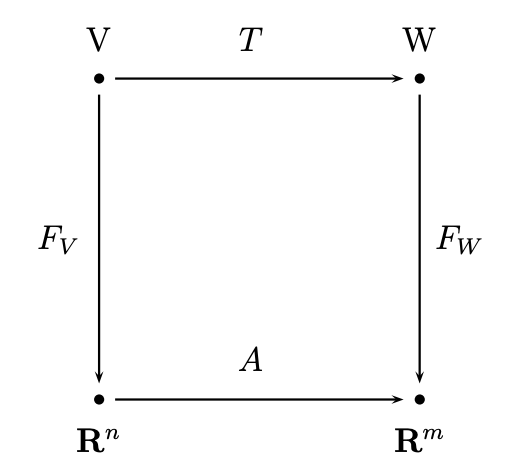
\includegraphics{visual}
Here are a few examples before proving it

\ex{}{
Let $T: P_1 \to P_2$ be the linear transformation defined by  $T(p(x)) = x(p(x))$ \\
Let us find the matrix which represents  $T$ with respect to bases  $B_1 = \{1,x\}$ and  $B_2 = \{1,x,x^2\}$ \\
We need to calculate  $[T(1)]_{B_2}$ and  $[T(x)]_{B_2}$ \\
$[T(1)]_{B_2} = [x]_{B_2} = \begin{pmatrix} 0 \\ 1 \\ 0 \end{pmatrix} $ and $[T(x)]_{B_2} = [x^2]_{B_2} = \begin{pmatrix} 0 \\ 0 \\ 1 \end{pmatrix} $
\\ Then $A = \begin{pmatrix} 0 & 0 \\ 1 & 0 \\ 0 & 1 \end{pmatrix} $
\\ To check, we will calculate $[T(ax+b)]_{S_2}$ and  $A[ax+b]_{S_1}$ separately (we should get the same answer) \\
Firstly  $T(ax+b) = x(ax+b) = ax^2 + bx \implies [T(ax+b)]_{B_2} = \begin{pmatrix} 0 \\ b \\ a \end{pmatrix} $ 
\\ Secondly, $A[ax+b]_{B_1} = \begin{pmatrix} 0 & 0 \\ 1 & 0 \\ 0 & 1 \end{pmatrix} \begin{pmatrix} b\\a \end{pmatrix} = \begin{pmatrix} 0 \\ b \\ a \end{pmatrix}  $

}
Now we prove this theorem:
\begin{myproof}
    Suppose $[\mathbf{v}]_{B_V} = \left( \lambda_1, \lambda_2, \cdots, \lambda_{n} \right) $, then \\
    $\mathbf{v} = \lambda_1 \mathbf{v}_1 + \lambda _2 \mathbf{v}_2 + \cdots + \lambda_{n}\mathbf{v}_{n}$ \\
    By the linearity of $T$, we get that:
    \\  $T(\mathbf{v}) = \lambda_1 T(\mathbf{v}_1) + \lambda _2 T(\mathbf{v}_2) + \cdots + \lambda_{n}T(\mathbf{v}_{n})$ 
    \[
    \begin{aligned}
        [T(\mathbf{v})]_{B_W}  & = \lambda_1 [T(\mathbf{v}_1)]_{B_W} + \lambda _2 [T(\mathbf{v}_2)]_{B_W} + \cdots + \lambda_{n}[T(\mathbf{v}_{n})]_{B_W}
        \\  & = A \begin{pmatrix} \lambda_1 \\ \lambda_2 \\ \vdots \\ \lambda_n  \end{pmatrix} 
    \end{aligned}
\]  \\ since $A$ has  $[T(\mathbf{v}_j)]_{B_W}$ for its columns and thus $[T(\mathbf{v})]_{B_W} = A[\mathbf{v}]_{B_V}$
    \\ Now we have that $[T(\mathbf{v})]_{B_W} = $
\end{myproof}

\ex{}{
    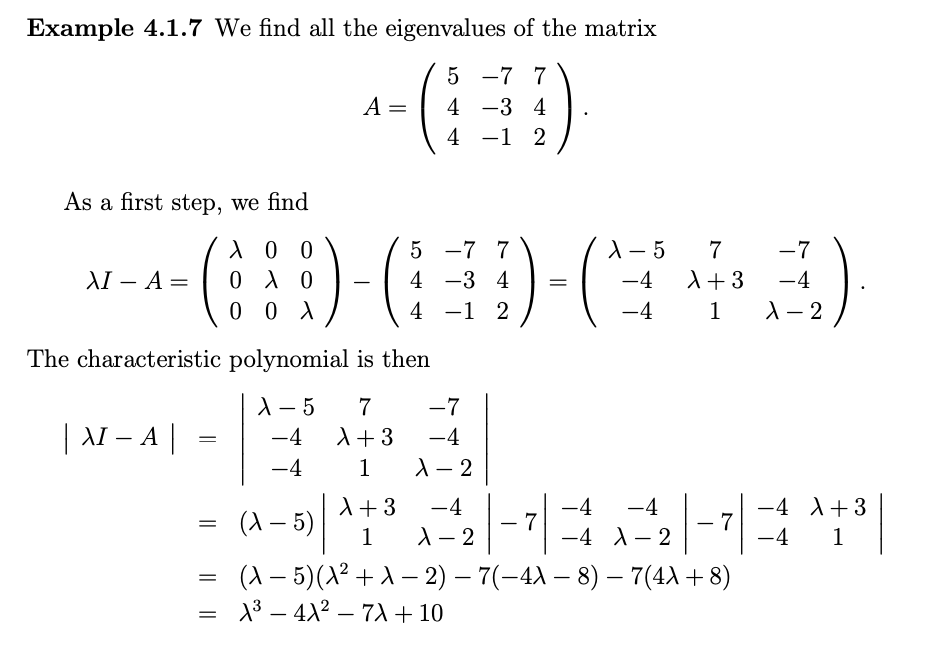
\includegraphics[scale = 0.9]{ex1} \\
    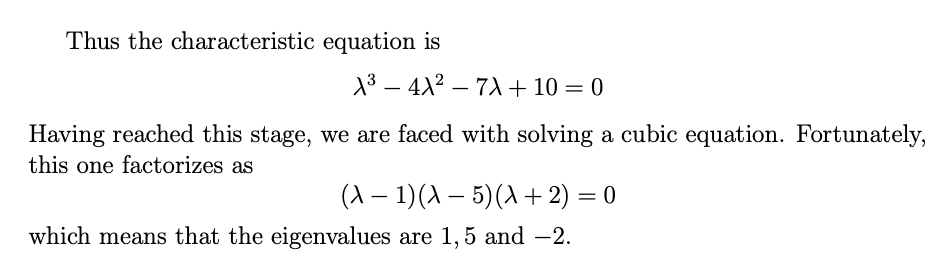
\includegraphics{ex2}
}

\thm{}{
Let $T:V \to W$ be a linear transformation and let  $V$ be finite dimensional. Then
 \begin{center}
    $\dim \left( \mathrm{ker}(T) \right) + \dim \left( \mathrm{ran}(T) \right) = \dim V $
\end{center}
}

\begin{myproof}
    Add in after (in tut)
\end{myproof}

\cor{}{
Let $V$ be a finite dimensional vector space and  $T:V \to V$ be a linear transformation. Then the following are equivalent:
 \begin{itemize}
    \item $T$ is injective
    \item  $T$ is surjective
    \item  $T$ is a linear isomorphism
\end{itemize}
}

\begin{myproof}
    Exercise. Use the facts that T is injective if and only if ker(T) = $\{0\}$ and
that for a subspace U of V we have dim U =dim V if and only if U = V .
\end{myproof}

\nt{
The above result shows that a linear function from a vector space into itself is
rather special: if it is either injective or surjective, then it will automatically be both
injective and surjective. Convince your self that this need not be true for non-linear
functions.
}
\end{document}
